\documentclass[tikz,border=2pt]{standalone}
\usepackage{amsmath,amssymb}
\usepackage{tikz}
\usetikzlibrary{arrows.meta}

\begin{document}
% Inside the radius of convergence the series converges pointwise on the open interval
% (a-R, a+R), and uniformly (also after differentiating term by term) on every closed
% sub-interval [a-r, a+r] with r < R.
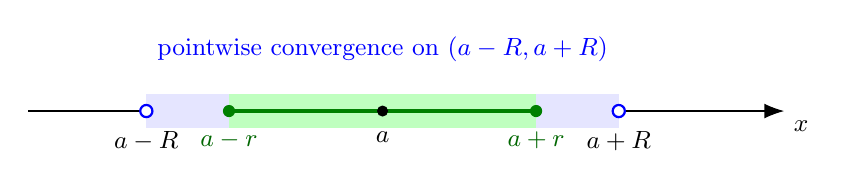
\begin{tikzpicture}[x=1.5cm, every node/.style={font=\small}]
	\draw[-{Latex[length=2.5mm]}] (-3,0) -- (3.4,0) node[below right] {$x$};
	\fill[blue!10] (-2,-0.22) rectangle (2,0.22);
	\fill[green!25] (-1.3,-0.22) rectangle (1.3,0.22);
	\draw[very thick, green!50!black] (-1.3,0) -- (1.3,0);
	\fill[green!50!black] (-1.3,0) circle (2.2pt);
	\fill[green!50!black] (1.3,0) circle (2.2pt);
	\draw[blue, thick, fill=white] (-2,0) circle (2.2pt);
	\draw[blue, thick, fill=white] (2,0) circle (2.2pt);
	\fill[black] (0,0) circle (2pt);
	\node[below=4pt] at (0,0) {$a$};
	\node[below=4pt] at (-2,0) {$a-R$};
	\node[below=4pt] at (2,0) {$a+R$};
	\node[below=4pt, green!40!black] at (-1.3,0) {$a-r$};
	\node[below=4pt, green!40!black] at (1.3,0) {$a+r$};
	\node[blue, above=8pt] at (0,0.22) {pointwise convergence on $(a-R,a+R)$};
\end{tikzpicture}
\end{document}
